\documentclass[11pt,a4paper,usenames,dvipsnames]{article}
\usepackage{url,amsmath,amssymb,latexsym,mathrsfs,comment,amsthm,enumerate,geometry,calc,ifthen,mathdots,textcomp,multicol}
\usepackage[colorlinks]{hyperref}
\usepackage[x11names, svgnames, rgb,table]{xcolor}
\usepackage{tikz-cd}
\usepackage[utf8]{inputenc}
\usepackage[T1]{fontenc}
\usepackage{tikz}
\usepgflibrary{snakes,arrows,shapes}
\pgfdeclarelayer{background layer}
\pgfsetlayers{background layer,main}
\usetikzlibrary{decorations.markings}
\usetikzlibrary{arrows,matrix}
\usepgflibrary{arrows}
\tikzset{->-/.style={decoration={
  markings,
  mark=at position #1 with {\arrow{{latex}}}},postaction={decorate}}}

\begin{document}

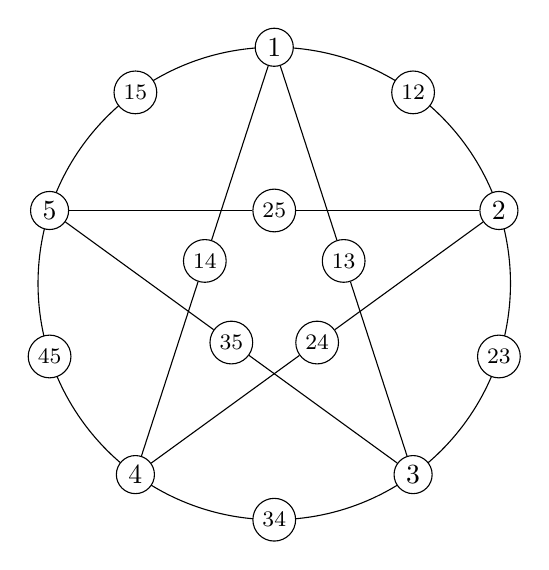
\begin{tikzpicture}[scale=3]
\tikzstyle{vertex}=[circle,draw=black, fill=white, inner sep = 0.07cm]
%
\draw (0,0) circle (1);
\node[vertex] (1) at (90:1) {  $1$ };
\node[vertex] (2) at (90-72:1) {  $2$ };
\node[vertex] (3) at (90-72-72:1) {  $3$ };
\node[vertex] (4) at (90-72-72-72:1) {  $4$ };
\node[vertex] (5) at (90-72-72-72-72:1) {  $5$ };
\node[vertex] (12) at (90-36:1) {\footnotesize  $12$ };
\node[vertex] (13) at (0.293890801	,0.095490177) {\footnotesize  $13$ };
\node[vertex] (14) at (-0.293894022	,0.095492517) {\footnotesize  $14$ };
\node[vertex] (15) at (90-36-72-72-72-72:1) {\footnotesize  $15$ };
\node[vertex] (23) at (90-36-72:1) {\footnotesize  $23$ };
\node[vertex] (24) at (0.181635098	,-0.250001636) {\footnotesize  $24$ };
\node[vertex] (25) at (0	,0.30901548) {\footnotesize  $25$ };
\node[vertex] (34) at (90-36-72-72:1) {\footnotesize  $34$ };
\node[vertex] (35) at (-0.181637088	,-0.25000019) {\footnotesize  $35$ };
\node[vertex] (45) at (90-36-72-72-72:1) {\footnotesize  $45$ };
%
\foreach \x/\y in {1/3,1/4,2/4,2/5,3/5} {\draw(\x)--(\x\y)--(\y);}
\end{tikzpicture}

\end{document}